% =============================================================
% CAPÍTULO 2 — Estado del arte y marco teórico
% =============================================================

\section{Estado del arte y marco teórico}
\label{sec:estado-arte}

Este capítulo proporciona los fundamentos teóricos y el contexto de investigación
necesarios para comprender el resto de la memoria. La exposición sigue un orden
constructivo: primero se traza la evolución del NLP hasta la arquitectura Transformer
(\S\ref{sec:sota-historia}); después se presenta el Transformer en detalle
(\S\ref{sec:sota-transformer}); a continuación se describe BERT
(\S\ref{sec:sota-bert}); se desarrollan los fundamentos matemáticos de la SVD
(\S\ref{sec:sota-svd-teoria}); se sitúa el problema de la clasificación de emociones
(\S\ref{sec:sota-emociones}); se revisan las técnicas de compresión
(\S\ref{sec:sota-compresion}); se presentan las herramientas de interpretabilidad
mecánica (\S\ref{sec:sota-interpretabilidad}); y se cierra con el posicionamiento
del trabajo (\S\ref{sec:sota-posicionamiento}).

% =============================================================
\subsection{Del procesamiento secuencial al Transformer}
\label{sec:sota-historia}
% =============================================================

El procesamiento del lenguaje natural fue durante décadas un problema fundamentalmente
secuencial. Las redes neuronales recurrentes (RNN) \cite{elman1990finding} procesaban
los tokens uno a uno, manteniendo un vector de estado oculto que acumulaba información
de los tokens anteriores. En la práctica, esta información se degradaba
exponencialmente con la distancia: las RNN sufrían el problema del
\emph{desvanecimiento del gradiente} \cite{bengio1994learning}, que impedía aprender
dependencias a larga distancia. Las LSTM \cite{hochreiter1997long} mitigaron
parcialmente este problema introduciendo mecanismos de puertas que controlan qué
información se almacena, se olvida o se transmite, y dominaron el NLP durante la
década de 2014--2017.

Sin embargo, las arquitecturas recurrentes tienen una limitación estructural: al
procesar los tokens secuencialmente, la computación no es paralelizable (el cálculo
de $h_t$ depende de $h_{t-1}$), lo que limita la velocidad de entrenamiento e impide
aprovechar eficientemente las GPUs.

Un primer avance fue el mecanismo de atención de Bahdanau et al.\
\cite{bahdanau2015neural}, que permitió al decoder de un modelo de traducción atender
selectivamente a distintas posiciones del encoder, eliminando el cuello de botella de
comprimir toda la frase de origen en un único vector. Pero la recurrencia seguía
presente.

La contribución de Vaswani et al.\ \cite{vaswani2017attention} fue radical: el
Transformer elimina completamente las operaciones recurrentes y se basa
exclusivamente en mecanismos de atención, logrando tres ventajas:

\begin{enumerate}[nosep]
    \item \textbf{Paralelismo total}: todas las posiciones se procesan simultáneamente.
    \item \textbf{Distancia constante}: la atención conecta cualquier par de posiciones
    en $O(1)$, frente a los $O(n)$ pasos de una RNN.
    \item \textbf{Escalabilidad}: permitió entrenar modelos significativamente más
    grandes, abriendo la puerta a los modelos de lenguaje pre-entrenados.
\end{enumerate}

El impacto fue inmediato en traducción automática, pero la revolución real vino
después: la arquitectura Transformer, pre-entrenada sobre grandes corpus, producía
representaciones lingüísticas de propósito general transferibles a prácticamente
cualquier tarea de NLP. Esto dio lugar a la era de los \textit{foundation models}
(BERT, GPT, T5).

% =============================================================
\subsection{La arquitectura Transformer}
\label{sec:sota-transformer}
% =============================================================

La arquitectura Transformer original \cite{vaswani2017attention} consta de dos
bloques apilados (encoder y decoder) conectados mediante atención cruzada
(Figura~\ref{fig:transformer-original}). El encoder procesa la secuencia de
entrada y produce representaciones contextualizadas; el decoder genera la secuencia
de salida de forma autoregresiva. BERT utiliza exclusivamente la torre del encoder,
descartando el decoder por completo, ya que su objetivo no es generar secuencias
sino producir representaciones bidireccionales reutilizables.

\begin{figure}[H]
    \centering
    \includegraphics[width=0.45\textwidth]{figures/transformer_original.png}
    \caption{Arquitectura Transformer original (Vaswani et al., 2017). El encoder
    (izquierda) y el decoder (derecha) se componen de bloques apilados $N$ veces.
    BERT utiliza exclusivamente la torre del encoder. Figura adaptada
    de~\cite{vaswani2017attention}.}
    \label{fig:transformer-original}
\end{figure}

La Figura~\ref{fig:bert-encoder} detalla la estructura interna de un bloque
encoder, que se apila 12 veces en BERT-base. El resto de esta sección describe
sus componentes.

\begin{figure}[H]
    \centering
    \shorthandoff{><}
    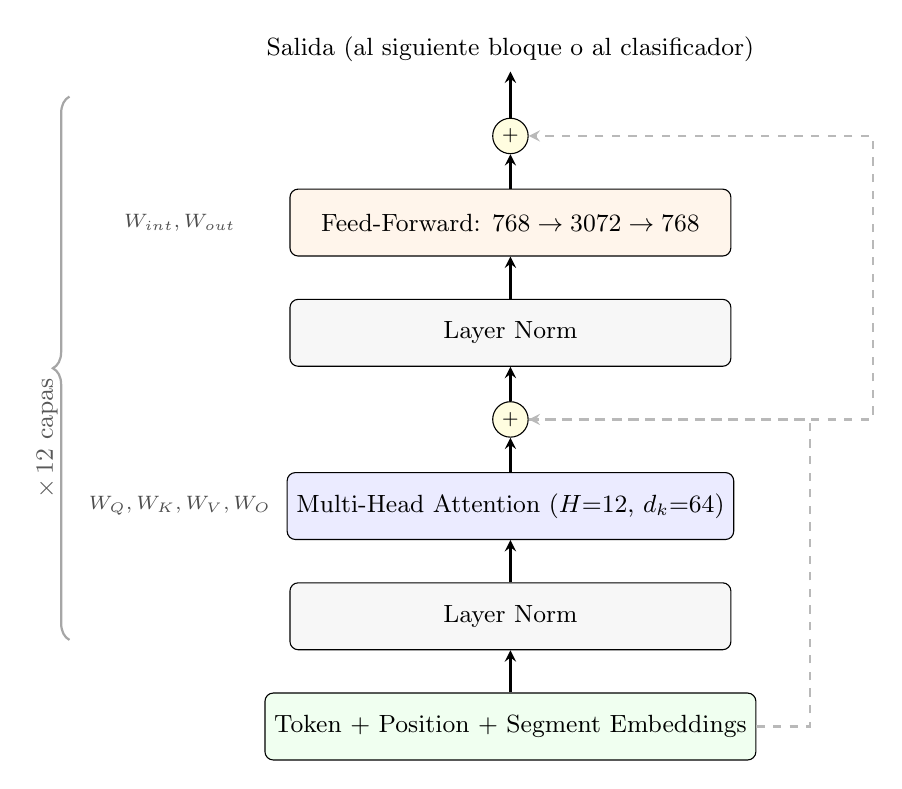
\begin{tikzpicture}[
        block/.style={draw, rounded corners=3pt, minimum height=0.85cm,
                      font=\small, minimum width=5.6cm, anchor=center},
        attn/.style={block, fill=blue!8},
        ffn/.style={block, fill=orange!8},
        norm/.style={block, fill=gray!6},
        emb/.style={block, fill=green!6},
        add/.style={draw, circle, minimum size=0.45cm, fill=yellow!12,
                    font=\scriptsize, inner sep=0pt},
        arr/.style={->, >=stealth, thick},
        res/.style={->, >=stealth, thick, dashed, gray!55},
        brace/.style={decorate, decoration={brace, amplitude=6pt}, thick, gray!70},
        lab/.style={font=\scriptsize, gray!60!black},
    ]
        % === Nodes ===
        \node[emb]  (emb)  at (0, 0.0) {Token + Position + Segment Embeddings};
        \node[norm] (ln1)  at (0, 1.4) {Layer Norm};
        \node[attn] (attn) at (0, 2.8) {Multi-Head Attention ($H{=}12$, $d_k{=}64$)};
        \node[add]  (add1) at (0, 3.9) {$+$};
        \node[norm] (ln2)  at (0, 5.0) {Layer Norm};
        \node[ffn]  (ffn)  at (0, 6.4) {Feed-Forward: $768 \rightarrow 3072 \rightarrow 768$};
        \node[add]  (add2) at (0, 7.5) {$+$};
        \node[font=\small] (out) at (0, 8.6) {Salida (al siguiente bloque o al clasificador)};

        % === Main vertical flow ===
        \draw[arr] (emb)  -- (ln1);
        \draw[arr] (ln1)  -- (attn);
        \draw[arr] (attn) -- (add1);
        \draw[arr] (add1) -- (ln2);
        \draw[arr] (ln2)  -- (ffn);
        \draw[arr] (ffn)  -- (add2);
        \draw[arr] (add2) -- (out);

        % === Residual 1: emb bypasses attn, joins at add1 ===
        \draw[res] (emb.east) -- (3.8, 0.0) -- (3.8, 3.9) -- (add1.east);

        % === Residual 2: add1 output bypasses ffn, joins at add2 ===
        \draw[res] (add1.east) -- (3.8, 3.9) -- (4.6, 3.9) -- (4.6, 7.5) -- (add2.east);

        % === Weight matrix annotations (left side) ===
        \node[lab] at (-4.2, 2.8) {$W_Q, W_K, W_V, W_O$};
        \node[lab] at (-4.2, 6.4) {$W_{\text{int}}, W_{\text{out}}$};

        % === Brace ===
        \draw[brace] (-5.6, 1.1) -- (-5.6, 8.0)
            node[midway, left=8pt, font=\small, gray!70!black, rotate=90]
            {$\times\, 12$ capas};
    \end{tikzpicture}
    \shorthandon{><}
    \caption{Arquitectura de un bloque encoder de BERT-base. Cada bloque contiene
    un sub-bloque de atención multi-cabeza (con 12 cabezas de dimensión 64) y un
    sub-bloque feed-forward (con expansión $768 \rightarrow 3072 \rightarrow 768$),
    ambos con conexión residual (líneas discontinuas) y layer normalization. Las 6
    matrices de pesos anotadas ($W_Q, W_K, W_V, W_O, W_{\text{int}}, W_{\text{out}}$)
    son el objetivo de la compresión SVD. BERT-base apila 12 de estos bloques.}
    \label{fig:bert-encoder}
\end{figure}

% -------------------------------------------------------------
\subsubsection{Atención multi-cabeza}
\label{sec:sota-mha}
% -------------------------------------------------------------

El mecanismo central del Transformer es la \emph{atención escalada por producto
punto}. Dada una secuencia de $n$ tokens representada como $X \in \mathbb{R}^{n
\times d}$, cada cabeza de atención $h$ (de un total de $H$) computa tres
proyecciones lineales:
\begin{equation}
    Q_h = X W_Q^h, \quad K_h = X W_K^h, \quad V_h = X W_V^h
    \label{eq:qkv}
\end{equation}
donde $W_Q^h, W_K^h, W_V^h \in \mathbb{R}^{d \times d_k}$ con $d_k = d/H$. La
\emph{Query} codifica qué busca cada token, la \emph{Key} codifica qué ofrece, y
el \emph{Value} contiene la información que se transmitirá.

La atención se computa en tres pasos. Primero, los scores de compatibilidad:
\begin{equation}
    S = \frac{Q_h K_h^T}{\sqrt{d_k}} \in \mathbb{R}^{n \times n}
    \label{eq:scores}
\end{equation}
El factor $1/\sqrt{d_k}$ evita que los productos punto crezcan con la dimensión,
estabilizando los gradientes a través de la softmax. Segundo, la normalización:
\begin{equation}
    A = \text{softmax}(S), \quad A_{ij} = \frac{e^{S_{ij}}}{\sum_{k=1}^{n} e^{S_{ik}}}
    \label{eq:softmax-attn}
\end{equation}
Cada fila $A_i$ es una distribución de probabilidad que determina cuánto atiende
el token $i$ a cada posición. Tercero, la salida como promedio ponderado de los
valores:
\begin{equation}
    \text{head}_h = A \cdot V_h \in \mathbb{R}^{n \times d_k}
    \label{eq:head-output}
\end{equation}

Las salidas de las $H$ cabezas se concatenan y se proyectan:
\begin{equation}
    \text{MultiHead}(X) = [\text{head}_1; \ldots; \text{head}_H]\, W_O
    \label{eq:multihead}
\end{equation}
donde $W_O \in \mathbb{R}^{d \times d}$. Cada cabeza opera en un subespacio de
dimensión $d_k$ y puede especializarse en un tipo diferente de relación entre
tokens. Investigaciones posteriores \cite{voita2019analyzing, clark2019what}
confirmaron que esta especialización emerge espontáneamente: algunas cabezas
atienden a posiciones sintácticas, otras a tokens semánticamente relacionados, y
otras a patrones posicionales fijos.

\begin{figure}[H]
    \centering
    \shorthandoff{><}
    \begin{tikzpicture}[
        block/.style={draw, rounded corners=2pt, minimum height=0.7cm, minimum width=1.4cm,
                      fill=blue!8, font=\small, anchor=center},
        op/.style={draw, circle, minimum size=0.55cm, fill=orange!12, font=\scriptsize,
                   inner sep=0pt},
        arr/.style={->, >=stealth, thick},
    ]
        % === Row 1: Input X (centered below projections) ===
        \node (X) at (1.8, 0) {$X$};

        % === Row 2: Linear projections ===
        \node[block] (WQ) at (0,   1.5) {$W_Q^h$};
        \node[block] (WK) at (1.8, 1.5) {$W_K^h$};
        \node[block] (WV) at (3.6, 1.5) {$W_V^h$};

        % === Row 3: Q, K, V labels ===
        \node[font=\small] (Q) at (0,   2.6) {$Q_h$};
        \node[font=\small] (K) at (1.8, 2.6) {$K_h$};
        \node[font=\small] (V) at (3.6, 2.6) {$V_h$};

        % === Row 4: MatMul Q·K^T ===
        \node[op] (mm1) at (0.9, 3.7) {$\times$};
        \node[font=\scriptsize, gray, right=0.7cm of mm1] {$QK^T\!/\!\sqrt{d_k}$};

        % === Row 5: Softmax ===
        \node[block, fill=green!8] (sm) at (0.9, 4.8) {softmax};

        % === Row 6: MatMul with V ===
        \node[op] (mm2) at (0.9, 5.9) {$\times$};

        % === Row 7: Output ===
        \node[font=\small] (out) at (0.9, 6.8) {$\text{head}_h$};

        % === Arrows: X to projections ===
        \draw[arr] (X) -- (WQ);
        \draw[arr] (X) -- (WK);
        \draw[arr] (X) -- (WV);

        % === Arrows: projections to labels ===
        \draw[arr] (WQ) -- (Q);
        \draw[arr] (WK) -- (K);
        \draw[arr] (WV) -- (V);

        % === Arrows: Q and K into mm1 ===
        \draw[arr] (Q) -- (0, 3.7) -- (mm1);
        \draw[arr] (K) -- (1.8, 3.7) -- (mm1);

        % === Arrow: mm1 to softmax to mm2 to output ===
        \draw[arr] (mm1) -- (sm);
        \draw[arr] (sm) -- (mm2);
        \draw[arr] (mm2) -- (out);

        % === Arrow: V bypasses to mm2 ===
        \draw[arr] (V) -- (3.6, 5.9) -- (mm2);
    \end{tikzpicture}
    \shorthandon{><}
    \caption{Mecanismo de atención para una cabeza $h$. La entrada $X$ se proyecta
    en Query, Key y Value. Los scores $QK^T/\sqrt{d_k}$ se normalizan con softmax
    y ponderan los valores para generar la salida.}
    \label{fig:attention-mechanism}
\end{figure}

% -------------------------------------------------------------
\subsubsection{El bloque feed-forward}
\label{sec:sota-ffn}
% -------------------------------------------------------------

Cada capa incluye un bloque feed-forward (FFN) que se aplica posición por posición:
\begin{equation}
    \text{FFN}(x) = \text{GELU}(x\, W_{\text{int}} + b_1)\, W_{\text{out}} + b_2
    \label{eq:ffn}
\end{equation}
donde $W_{\text{int}} \in \mathbb{R}^{d \times d_{ff}}$ y $W_{\text{out}} \in
\mathbb{R}^{d_{ff} \times d}$, con $d_{ff} = 4d = 3072$ en BERT-base. La función
de activación GELU (\textit{Gaussian Error Linear Unit}) \cite{hendrycks2016gaussian}
se define como:
\begin{equation}
    \text{GELU}(x) = x \cdot \Phi(x) \approx 0{,}5\, x \left(1 + \tanh\!\left[\sqrt{2/\pi}\,(x + 0{,}044715\, x^3)\right]\right)
    \label{eq:gelu}
\end{equation}
donde $\Phi(x)$ es la función de distribución acumulada de la normal estándar. A
diferencia de ReLU, GELU es suave y permite gradientes no-nulos para valores negativos
pequeños. Esta no-linealidad entre $W_{\text{int}}$ y $W_{\text{out}}$ es lo que
convierte a la FFN en un bloque computacional genuino: sin ella, las dos
multiplicaciones matriciales colapsarían en una sola transformación lineal.

La dimensión
intermedia expandida crea un espacio de representación cuatro veces mayor que el
espacio residual, donde el modelo puede computar transformaciones complejas antes de
proyectar de vuelta. Geva et al.\ \cite{geva2021transformer} propusieron que las
neuronas de esta capa funcionan como \emph{memorias clave-valor}: cada neurona
almacena un patrón de activación (clave, en $W_{\text{int}}$) y un vector de
actualización del espacio residual (valor, en $W_{\text{out}}$). Esta perspectiva
es directamente relevante para el análisis de especialización neuronal emocional
del Capítulo~\ref{sec:resultados-interpretabilidad}.

% -------------------------------------------------------------
\subsubsection{Conexiones residuales y flujo residual}
\label{sec:sota-residual}
% -------------------------------------------------------------

El output de cada sub-bloque se combina con su input mediante una \emph{conexión
residual} \cite{he2016deep} seguida de \emph{layer normalization} \cite{ba2016layer}:
\begin{align}
    h'  &= \text{LayerNorm}(x + \text{MultiHead}(x)) \label{eq:residual-attn} \\
    h'' &= \text{LayerNorm}(h' + \text{FFN}(h')) \label{eq:residual-ffn}
\end{align}

Las conexiones residuales crean un \emph{flujo residual} (\textit{residual stream})
que atraviesa todas las capas. Elhage et al.\ \cite{elhage2021mathematical}
formalizaron esta perspectiva: conceptualmente, cada capa lee del flujo, computa una
actualización, y la escribe de vuelta sumándola. La representación final de un token
es la suma acumulada de todas las contribuciones:
\begin{equation}
    x_L = x_0 + \sum_{l=1}^{L} \Delta_l^{\text{attn}} + \sum_{l=1}^{L} \Delta_l^{\text{ffn}}
    \label{eq:residual-stream}
\end{equation}

Esta arquitectura tiene una implicación crucial para la compresión: cuando se comprime
una capa intermedia, la señal corrupta se propaga por el flujo residual a todas las
capas posteriores, generando un \emph{efecto cascada} que amplifica el daño.

% =============================================================
\subsection{BERT}
\label{sec:sota-bert}
% =============================================================

BERT (\textit{Bidirectional Encoder Representations from Transformers})
\cite{devlin2019bert} demostró el poder del paradigma \textit{pre-train + fine-tune}:
un Transformer encoder pre-entrenado sobre grandes corpus produce representaciones
transferibles a tareas específicas con un \emph{fine-tuning} mínimo.

BERT-base consta de $L = 12$ capas de encoder, con $d = 768$, $H = 12$ cabezas
($d_k = 64$), y $d_{ff} = 3072$, sumando 110 millones de parámetros. De estos,
84{,}9 millones corresponden a las 72 capas lineales del encoder (6 matrices por
capa $\times$ 12 capas), que son el objetivo de la compresión SVD.

% -------------------------------------------------------------
\subsubsection{Pre-entrenamiento bidireccional}
\label{sec:sota-bert-pretraining}
% -------------------------------------------------------------

BERT se pre-entrena sobre BookCorpus + Wikipedia (3.300 millones de palabras)
mediante \textit{Masked Language Modeling} (MLM): se enmascara aleatoriamente
el 15\% de los tokens y el modelo debe predecirlos a partir del contexto
bidireccional. A diferencia de los modelos autoregresivos como GPT
\cite{radford2018improving}, que solo ven el contexto izquierdo, BERT accede
simultáneamente al contexto izquierdo y derecho, lo que produce representaciones
más ricas. Para la clasificación de emociones, donde el tono emocional puede
depender de partículas negativas al final de la frase (``no estoy enfadado
en absoluto''), esta bidireccionalidad es especialmente valiosa.

BERT también incluye un segundo objetivo de pre-entrenamiento, \textit{Next Sentence
Prediction} (NSP), que entrena al modelo a predecir si dos frases son consecutivas
en el texto original. Aunque trabajos posteriores como RoBERTa \cite{liu2019roberta}
demostraron que NSP no es necesario e incluso puede ser contraproducente, forma
parte del diseño original de BERT-base, que es el modelo utilizado en este trabajo.

\begin{figure}[H]
    \centering
    \shorthandoff{><}
    \begin{tikzpicture}[
        tok/.style={draw, rounded corners=2pt, minimum height=0.65cm, minimum width=1.3cm,
                    font=\small},
        inp/.style={tok, fill=blue!6},
        mask/.style={tok, fill=red!12},
        pred/.style={tok, fill=green!10, dashed},
        arr/.style={->, >=stealth, thick, gray},
    ]
        \node[inp] (t1) at (0,0) {\texttt{[CLS]}};
        \node[inp] (t2) at (1.6,0) {I};
        \node[inp] (t3) at (3.2,0) {really};
        \node[mask] (t4) at (4.8,0) {\texttt{[MASK]}};
        \node[inp] (t5) at (6.4,0) {this};
        \node[inp] (t6) at (8.0,0) {movie};

        \node[draw, thick, rounded corners, fill=gray!4, minimum width=9.8cm,
              minimum height=1.0cm, font=\small] (bert) at (4.0, 1.4) {BERT Encoder (12 capas)};

        \node[pred] (p4) at (4.8, 2.8) {love};

        \foreach \i in {t1,t2,t3,t4,t5,t6} {
            \draw[arr] (\i.north) -- (\i.north |- bert.south);
        }
        \draw[arr, thick, green!50!black] (bert.north -| t4) -- (p4.south);

        \node[font=\scriptsize, red!60!black, below=0.08cm of t4] {enmascarado};
        \node[font=\scriptsize, green!50!black, above=0.08cm of p4] {predecir original};
    \end{tikzpicture}
    \shorthandon{><}
    \caption{Masked Language Modeling. El modelo predice los tokens enmascarados
    usando el contexto bidireccional completo.}
    \label{fig:mlm}
\end{figure}

% -------------------------------------------------------------
\subsubsection{El token \texttt{[CLS]} y el \emph{fine-tuning}}
\label{sec:sota-cls}
% -------------------------------------------------------------

BERT añade un token especial \texttt{[CLS]} al inicio de cada secuencia. Al no
corresponder a ninguna palabra real, \texttt{[CLS]} no tiene significado léxico
propio y funciona como recolector de información global: a lo largo de las 12 capas,
acumula información de toda la secuencia a través del mecanismo de atención. Su
representación en la última capa se usa como input al clasificador de la tarea.

El \emph{fine-tuning} consiste en añadir una capa lineal sobre \texttt{[CLS]} y entrenar
el modelo completo sobre la tarea objetivo. Esto transfiere el conocimiento
lingüístico del pre-entrenamiento a la tarea específica con un coste
significativamente menor que entrenar desde cero.

La propiedad de \texttt{[CLS]} como agregador lo convierte en el punto de lectura
natural para los \textit{probing classifiers} de este trabajo: su activación en
cada capa intermedia captura el estado de procesamiento del modelo en ese punto de
la jerarquía.

% =============================================================
\subsection{Fundamentos de la descomposición en valores singulares}
\label{sec:sota-svd-teoria}
% =============================================================

La SVD es la herramienta matemática central de este proyecto. Esta sección
desarrolla sus fundamentos teóricos y la intuición geométrica que conecta la
estructura espectral con la función computacional.

% -------------------------------------------------------------
\subsubsection{Definición y propiedades}
\label{sec:sota-svd-definicion}
% -------------------------------------------------------------

Toda matriz $W \in \mathbb{R}^{m \times n}$ admite una descomposición:
\begin{equation}
    W = U \Sigma V^T
    \label{eq:svd-completa}
\end{equation}
donde $U \in \mathbb{R}^{m \times m}$ y $V \in \mathbb{R}^{n \times n}$ son
matrices ortogonales, y $\Sigma \in \mathbb{R}^{m \times n}$ tiene los
\emph{valores singulares} $\sigma_1 \geq \sigma_2 \geq \cdots \geq \sigma_r > 0$
en la diagonal ($r = \text{rank}(W)$).

Las columnas de $U$ (\emph{vectores singulares izquierdos}) forman una base del
espacio de salida; las de $V$ (\emph{vectores singulares derechos}), del espacio de
entrada. Los valores singulares cuantifican la ganancia de la transformación en
cada dirección. Se relacionan con los autovalores de $W^T W$ mediante:
\begin{equation}
    \sigma_i = \sqrt{\lambda_i(W^T W)}
    \label{eq:svd-eigenvalues}
\end{equation}

% -------------------------------------------------------------
\subsubsection{Interpretación geométrica}
\label{sec:sota-svd-geometria}
% -------------------------------------------------------------

La SVD descompone cualquier transformación lineal en tres operaciones elementales:
$V^T$ rota el espacio de entrada alineando los ejes con las direcciones naturales
de la transformación; $\Sigma$ escala cada eje por su valor singular; y $U$ rota
el resultado al espacio de salida. Visualmente, $W$ convierte la esfera unitaria
en un elipsoide cuyos semiejes tienen longitudes $\sigma_1, \sigma_2, \ldots$

\begin{figure}[H]
    \centering
    \shorthandoff{><}
    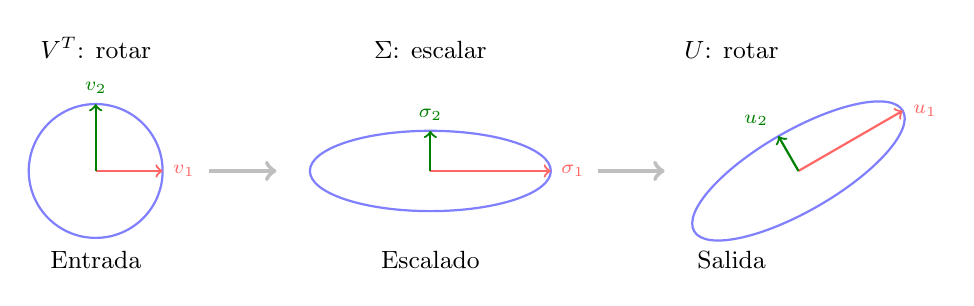
\begin{tikzpicture}[scale=0.85]
        % Unit circle
        \begin{scope}[shift={(-4,0)}]
            \draw[thick, blue!50] (0,0) circle (1);
            \draw[->, thick, red!60] (0,0) -- (1,0) node[right, font=\scriptsize] {$v_1$};
            \draw[->, thick, green!50!black] (0,0) -- (0,1) node[above, font=\scriptsize] {$v_2$};
            \node[below=0.9cm, font=\small] {Entrada};
            \node[above=1.3cm, font=\small] {$V^T$: rotar};
        \end{scope}

        \draw[->, ultra thick, gray!50] (-2.3,0) -- (-1.3,0);

        \begin{scope}[shift={(1,0)}]
            \draw[thick, blue!50] (0,0) ellipse (1.8 and 0.6);
            \draw[->, thick, red!60] (0,0) -- (1.8,0) node[right, font=\scriptsize] {$\sigma_1$};
            \draw[->, thick, green!50!black] (0,0) -- (0,0.6) node[above, font=\scriptsize] {$\sigma_2$};
            \node[below=0.9cm, font=\small] {Escalado};
            \node[above=1.3cm, font=\small] {$\Sigma$: escalar};
        \end{scope}

        \draw[->, ultra thick, gray!50] (3.5,0) -- (4.5,0);

        \begin{scope}[shift={(6.5,0)}, rotate=30]
            \draw[thick, blue!50] (0,0) ellipse (1.8 and 0.6);
            \draw[->, thick, red!60] (0,0) -- (1.8,0) node[right, font=\scriptsize] {$u_1$};
            \draw[->, thick, green!50!black] (0,0) -- (0,0.6) node[above left, font=\scriptsize] {$u_2$};
        \end{scope}
        \node[below=0.9cm, font=\small] at (5.5,0) {Salida};
        \node[above=1.3cm, font=\small] at (5.5,0) {$U$: rotar};
    \end{tikzpicture}
    \shorthandon{><}
    \caption{Interpretación geométrica de la SVD. La transformación $W$ convierte la
    esfera unitaria en un elipsoide mediante rotación ($V^T$), escalado ($\Sigma$)
    y rotación ($U$). Los semiejes del elipsoide son los valores singulares.}
    \label{fig:svd-geometric}
\end{figure}

En el contexto de BERT, las direcciones con valores singulares grandes corresponden
a las transformaciones que el modelo utiliza con más intensidad. Las de valores
pequeños pueden representar ruido, redundancia, o señales funcionales codificadas
con baja energía pero alta relevancia.

% -------------------------------------------------------------
\subsubsection{Aproximación de bajo rango y el teorema de Eckart-Young}
\label{sec:sota-eckart-young}
% -------------------------------------------------------------

La \emph{aproximación truncada de rango $k$} conserva los $k$ primeros valores
singulares:
\begin{equation}
    W_k = U_k \Sigma_k V_k^T = \sum_{i=1}^{k} \sigma_i\, u_i v_i^T
    \label{eq:svd-truncada-teoria}
\end{equation}

El \emph{teorema de Eckart-Young-Mirsky} \cite{eckart1936approximation} establece
que esta aproximación es óptima bajo la norma de Frobenius:
\begin{equation}
    W_k = \arg\min_{\text{rank}(\hat{W}) \leq k} \| W - \hat{W} \|_F
    \label{eq:eckart-young}
\end{equation}
con error:
\begin{equation}
    \| W - W_k \|_F^2 = \sum_{i=k+1}^{r} \sigma_i^2
    \label{eq:error-svd}
\end{equation}

Intuitivamente, la optimalidad se debe a que la norma de Frobenius es invariante
bajo rotaciones ortogonales ($\|W\|_F^2 = \sum_i \sigma_i^2$), de modo que retener
los $k$ valores singulares más grandes maximiza la energía capturada.

Sin embargo, la optimalidad es respecto a una métrica algebraica, no funcional. Dos
matrices con el mismo error de Frobenius pueden producir efectos radicalmente
distintos en el rendimiento del modelo, dependiendo de si los valores singulares
eliminados codifican redundancia o información crítica. Esta discrepancia es lo que
motiva el uso de interpretabilidad para guiar la compresión.

% -------------------------------------------------------------
\subsubsection{Energía espectral y compresión efectiva}
\label{sec:sota-energia-espectral}
% -------------------------------------------------------------

La fracción de energía retenida mide la calidad de la aproximación:
\begin{equation}
    E(k) = \frac{\sum_{i=1}^{k} \sigma_i^2}{\sum_{i=1}^{r} \sigma_i^2}
    \label{eq:energia}
\end{equation}

Matrices con decaimiento espectral rápido admiten compresión agresiva; matrices
con espectro plano resisten cualquier truncamiento.

\begin{figure}[H]
    \centering
    \shorthandoff{><}
    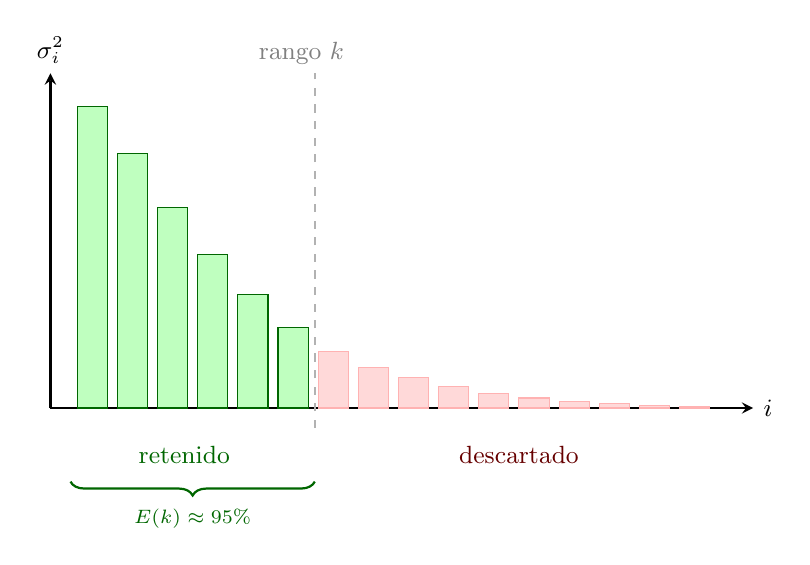
\begin{tikzpicture}[scale=0.85]
        \draw[->, >=stealth, thick] (0,0) -- (10.5,0) node[right, font=\small] {$i$};
        \draw[->, >=stealth, thick] (0,0) -- (0,5) node[above, font=\small] {$\sigma_i^2$};

        % Retained
        \foreach \x/\h in {0.4/4.5, 1.0/3.8, 1.6/3.0, 2.2/2.3, 2.8/1.7, 3.4/1.2} {
            \fill[green!25] (\x,0) rectangle (\x+0.45, \h);
            \draw[green!40!black] (\x,0) rectangle (\x+0.45, \h);
        }
        % Discarded
        \foreach \x/\h in {4.0/0.85, 4.6/0.6, 5.2/0.45, 5.8/0.32, 6.4/0.22, 7.0/0.15, 7.6/0.1, 8.2/0.07, 8.8/0.04, 9.4/0.02} {
            \fill[red!15] (\x,0) rectangle (\x+0.45, \h);
            \draw[red!30] (\x,0) rectangle (\x+0.45, \h);
        }

        \draw[dashed, thick, gray!60] (3.95, -0.3) -- (3.95, 5.0);
        \node[font=\small, gray] at (3.75, 5.3) {rango $k$};
        \node[font=\small, green!40!black] at (2.0, -0.7) {retenido};
        \node[font=\small, red!40!black] at (7.0, -0.7) {descartado};

        \draw[decorate, decoration={brace, amplitude=5pt, mirror}, thick, green!40!black]
            (0.3, -1.1) -- (3.95, -1.1) node[midway, below=6pt, font=\scriptsize] {$E(k) \approx 95\%$};
    \end{tikzpicture}
    \shorthandon{><}
    \caption{Espectro de valores singulares y truncamiento. Los primeros $k$ valores
    singulares capturan la mayor parte de la energía. La pregunta central de este
    trabajo es si la energía descartada contiene redundancia o señal funcional.}
    \label{fig:svd-spectrum}
\end{figure}

En la práctica, la aproximación reemplaza una capa $W$ de dimensión $m \times n$
por dos capas: $V_k^T$ ($k \times n$) y $U_k \Sigma_k$ ($m \times k$), reduciendo
los parámetros de $mn$ a $k(m+n)$. La compresión solo es efectiva cuando
$k < mn/(m+n)$, lo que da rangos de break-even de 384 para las matrices de atención
($768 \times 768$) y 614 para las FFN ($768 \times 3072$).

% =============================================================
\subsection{Clasificación de emociones en NLP}
\label{sec:sota-emociones}
% =============================================================

% -------------------------------------------------------------
\subsubsection{Del análisis de sentimientos a la detección de emociones}
\label{sec:sota-sentiment}
% -------------------------------------------------------------

El análisis de sentimientos, clasificar textos como positivos, negativos o
neutros \cite{pang2008opinion}, fue una de las primeras aplicaciones exitosas
del NLP, pero su granularidad de tres categorías es insuficiente para muchas
aplicaciones. La \emph{detección de emociones} aborda esta limitación usando
taxonomías más ricas, como las seis emociones básicas de Ekman
\cite{ekman1992argument} o el modelo de ocho emociones de Plutchik
\cite{plutchik1980general}. El dataset GoEmotions \cite{demszky2020goemotions},
con 28 categorías emocionales (27 emociones + \textit{neutral}) sobre 58.009
comentarios de Reddit, representa el estándar actual para esta tarea.

% -------------------------------------------------------------
\subsubsection{Clasificación multi-etiqueta}
\label{sec:sota-multilabel}
% -------------------------------------------------------------

Un mismo texto puede expresar múltiples emociones simultáneamente, lo que convierte
el problema en \emph{clasificación multi-etiqueta}. A diferencia de la clasificación
multi-clase, donde softmax distribuye una probabilidad total de 1 entre las clases
(forzando que una domine), la clasificación multi-etiqueta aplica sigmoid a cada
clase independientemente, permitiendo múltiples clases activas. La función de
pérdida correspondiente es la \emph{binary cross-entropy}:
\begin{equation}
    \mathcal{L} = -\frac{1}{C} \sum_{c=1}^{C} \left[ y_c \log(\hat{p}_c) + (1 - y_c) \log(1 - \hat{p}_c) \right]
    \label{eq:bce}
\end{equation}
donde $C = 23$, $y_c \in \{0, 1\}$, y $\hat{p}_c = \sigma(z_c)$.

\begin{figure}[H]
    \centering
    \shorthandoff{><}
    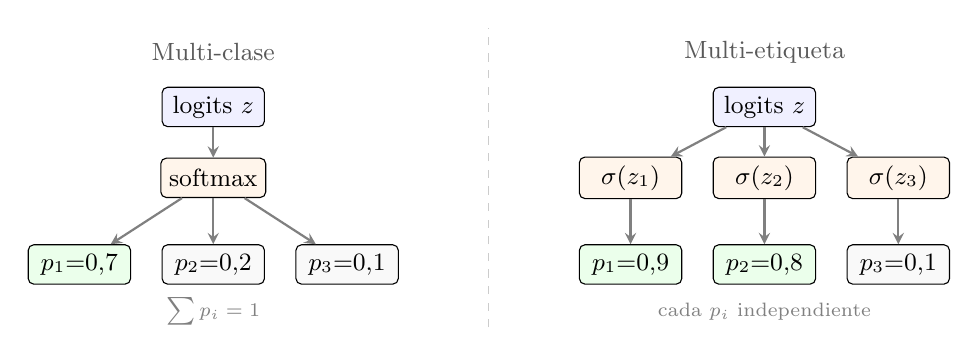
\begin{tikzpicture}[
        box/.style={draw, rounded corners=2pt, minimum height=0.5cm,
                    minimum width=1.3cm, font=\small, inner sep=3pt},
        arr/.style={->, >=stealth, thick, gray},
    ]
        % Multi-class
        \node[font=\small, gray!70!black] at (-3.5, 2.8) {Multi-clase};
        \node[box, fill=blue!6] (mc-logit) at (-3.5, 2.1) {logits $z$};
        \node[box, fill=orange!8] (mc-soft) at (-3.5, 1.2) {softmax};
        \node[box, fill=green!8] (mc-p1) at (-5.2, 0.1) {\small $p_1{=}0{,}7$};
        \node[box, fill=gray!5] (mc-p2) at (-3.5, 0.1) {\small $p_2{=}0{,}2$};
        \node[box, fill=gray!5] (mc-p3) at (-1.8, 0.1) {\small $p_3{=}0{,}1$};
        \node[font=\scriptsize, gray] at (-3.5, -0.5) {$\sum p_i = 1$};

        \draw[arr] (mc-logit) -- (mc-soft);
        \draw[arr] (mc-soft) -- (mc-p1);
        \draw[arr] (mc-soft) -- (mc-p2);
        \draw[arr] (mc-soft) -- (mc-p3);

        % Multi-label
        \node[font=\small, gray!70!black] at (3.5, 2.8) {Multi-etiqueta};
        \node[box, fill=blue!6] (ml-logit) at (3.5, 2.1) {logits $z$};
        \node[box, fill=orange!8] (ml-s1) at (1.8, 1.2) {$\sigma(z_1)$};
        \node[box, fill=orange!8] (ml-s2) at (3.5, 1.2) {$\sigma(z_2)$};
        \node[box, fill=orange!8] (ml-s3) at (5.2, 1.2) {$\sigma(z_3)$};
        \node[box, fill=green!8] (ml-p1) at (1.8, 0.1) {\small $p_1{=}0{,}9$};
        \node[box, fill=green!8] (ml-p2) at (3.5, 0.1) {\small $p_2{=}0{,}8$};
        \node[box, fill=gray!5] (ml-p3) at (5.2, 0.1) {\small $p_3{=}0{,}1$};
        \node[font=\scriptsize, gray] at (3.5, -0.5) {cada $p_i$ independiente};

        \draw[arr] (ml-logit) -- (ml-s1);
        \draw[arr] (ml-logit) -- (ml-s2);
        \draw[arr] (ml-logit) -- (ml-s3);
        \draw[arr] (ml-s1) -- (ml-p1);
        \draw[arr] (ml-s2) -- (ml-p2);
        \draw[arr] (ml-s3) -- (ml-p3);

        \draw[dashed, gray!40] (0, -0.7) -- (0, 3.1);
    \end{tikzpicture}
    \shorthandon{><}
    \caption{Multi-clase vs.\ multi-etiqueta. Softmax fuerza que una clase domine;
    sigmoid permite múltiples clases activas simultáneamente.}
    \label{fig:multiclass-multilabel}
\end{figure}

% -------------------------------------------------------------
\subsubsection{Desafíos de la clasificación emocional}
\label{sec:sota-desafios}
% -------------------------------------------------------------

La clasificación de emociones presenta desafíos específicos relevantes para
interpretar los resultados de este proyecto:

\paragraph{Ambigüedad semántica.}
Emociones como \textit{annoyance} y \textit{anger} ocupan regiones cercanas del
espacio semántico y se distinguen solo por intensidad o contexto pragmático. Esta
ambigüedad explica por qué algunas emociones necesitan más capas de procesamiento:
el modelo debe integrar información contextual que las primeras capas no capturan.

\paragraph{Desequilibrio de clases.}
En GoEmotions, \textit{admiration} tiene 4.130 ejemplos mientras que
\textit{embarrassment} tiene 303, un factor de 13{,}6$\times$. Este
desequilibrio afecta tanto al rendimiento como a la robustez frente a la compresión.

\paragraph{Señal léxica vs.\ contextual.}
Algunas emociones tienen marcadores léxicos claros (``gracias'' $\rightarrow$
\textit{gratitude}), mientras que otras dependen enteramente del contexto. Esta
distinción, que el probing captura como cristalización temprana vs.\ tardía, tiene
consecuencias directas para la compresión: las emociones léxicas son robustas
(su señal se captura en capas tempranas, redundantes y compresibles), mientras que
las contextuales dependen de las capas tardías (frágiles bajo SVD).

% =============================================================
\subsection{Compresión de modelos Transformer}
\label{sec:sota-compresion}
% =============================================================

La compresión de modelos busca reducir el tamaño y el coste computacional sin
destruir lo aprendido \cite{ganesh2021compressing}. En el contexto de los
Transformers, esto es especialmente relevante para el despliegue en entornos con
restricciones de memoria, latencia o energía \cite{strubell2019energy}.

\subsubsection{Poda}

La poda elimina pesos o estructuras completas cuya contribución es marginal
\cite{han2015deep}. Wang et al.\ \cite{wang2019structured} mostraron que es posible
eliminar hasta el 40\% de las cabezas de BERT sin pérdida significativa. Michel
et al.\ \cite{michel2019sixteen} confirmaron que en muchos casos una sola cabeza
por capa es suficiente. El inconveniente es que típicamente requiere re-entrenamiento.

\subsubsection{Cuantización}

La cuantización reduce la precisión numérica de los pesos (de float32 a int8 o
menos) \cite{jacob2018quantization}. Dettmers et al.\ \cite{dettmers2023qlora}
combinaron cuantización a 4 bits con adaptadores de bajo rango (QLoRA). La
limitación es la dependencia de hardware con soporte para operaciones de baja
precisión.

\subsubsection{Destilación}

En la destilación, un modelo pequeño aprende a imitar a uno grande. DistilBERT
\cite{sanh2019distilbert} redujo BERT a 6 capas conservando el 97\% del
rendimiento. El coste es un ciclo completo de entrenamiento.

\subsubsection{Factorización de bajo rango}

La SVD (\S\ref{sec:sota-svd-teoria}) es el método más directo. Noach y Goldberg
\cite{noach2020compressing} la aplicaron a BERT con compresión uniforme. Hsu et al.\
\cite{hsu2022language} propusieron una variante ponderada por la información de
Fisher que prioriza las direcciones más relevantes para la tarea. LoRA
\cite{hu2022lora} aborda el problema inverso: en lugar de comprimir un modelo
existente, añade adaptadores de bajo rango para \emph{fine-tuning} eficiente. La
literatura ha analizado también las propiedades estructurales de bajo rango en
los Transformers desde dos ángulos complementarios: Bhojanapalli et
al.~\cite{bhojanapalli2020low} demostraron que las cabezas de atención presentan
un \emph{cuello de botella de bajo rango} cuando la dimensión por cabeza es
inferior a la longitud de secuencia, resultado que conecta directamente con la
asimetría espectral entre componentes Q/K y FFN documentada en este trabajo. Por su parte,
Wang et al.~\cite{wang2020linformer} (Linformer) explotaron explícitamente la
naturaleza intrínsecamente de bajo rango de la matriz de atención
$\text{softmax}(QK^T)$ para reducir su complejidad de $O(n^2)$ a $O(n)$. Estos
trabajos sugieren que la atención es estructuralmente comprimible, lo que es
consistente con la robustez de Q/K bajo SVD que documentaremos en el
Capítulo~\ref{sec:resultados-compresion}.

La línea de SVD para LLMs ha continuado activa en 2023--2024.
ASVD~\cite{yuan2023asvd} introduce una variante consciente de las
activaciones que pondera los valores singulares por la magnitud de las
activaciones de entrada típicas, mejorando la fidelidad respecto a la
SVD ingenua sobre LLaMA-7B y similares. SVD-LLM~\cite{wang2024svdllm}
incorpora una corrección \emph{truncation-aware} que minimiza el error
en el espacio de salida y reporta resultados competitivos hasta el 60\%
de compresión. ShortGPT~\cite{men2024shortgpt} aborda una pregunta
ortogonal pero relacionada ---qué \emph{capas enteras} son
prescindibles--- y muestra que en LLaMA-2-13B se pueden eliminar hasta
9~de las 40~capas con caída moderada. Otra línea relacionada,
SparseGPT~\cite{frantar2023sparsegpt}, demuestra que la poda no
estructurada \emph{one-shot} sin re-entrenamiento es viable a escala
de 175\,000~M de parámetros. La Tabla~\ref{tab:comparativa-tecnicas}
resume las características de las cinco familias de técnicas; los
trabajos recientes sobre SVD para LLMs operan dentro de la familia
``SVD'' pero con variantes algorítmicas más sofisticadas que la
truncación clásica empleada en este TFG.

\begin{table}[H]
    \centering
    \caption{Comparativa de técnicas de compresión para Transformers.}
    \label{tab:comparativa-tecnicas}
    \small
    \begin{tabular}{@{}l c c c c c@{}}
        \toprule
        & \textbf{Poda} & \textbf{Cuantiz.} & \textbf{Destilación} & \textbf{SVD} & \textbf{LoRA} \\
        \midrule
        Re-entrenamiento      & Sí/Parcial & No/Parcial & Sí (completo) & No\textsuperscript{*}   & Sí (parcial) \\
        Granularidad          & Media       & Baja       & Baja          & Alta & Alta \\
        Garantías teóricas    & No          & Parcial    & No            & Sí   & Parcial \\
        Aplicable post-hoc    & Parcial     & Sí         & No            & Sí   & No \\
        Hardware especial     & No          & Sí         & No            & No   & No \\
        \bottomrule
    \end{tabular}
    \\[0.15cm]{\scriptsize \textsuperscript{*}No requiere re-entrenamiento para
    su aplicación inicial; el efecto de un \emph{fine-tuning} posterior se evalúa
    empíricamente en el Capítulo~\ref{sec:sintesis}.}
\end{table}

\subsubsection{Justificación del enfoque SVD}

La SVD encaja con los objetivos de este proyecto por cuatro razones: no requiere
re-entrenamiento para su aplicación, lo que permite evaluar decenas de
configuraciones a coste computacional bajo y desacoplar el efecto de la
compresión del efecto del re-entrenamiento; ofrece granularidad máxima
(rango específico por capa); el teorema de Eckart-Young
(\S\ref{sec:sota-eckart-young}) proporciona garantías de optimalidad respecto a
la norma de Frobenius; y el espectro de valores singulares aporta
interpretabilidad directa sobre la estructura de cada matriz de pesos. La
posibilidad de combinar la SVD con un \emph{fine-tuning} posterior se evalúa
empíricamente en el Capítulo~\ref{sec:sintesis}.

Un aspecto común a todas las técnicas anteriores es que son \emph{ciegas} respecto
a la función del modelo: la poda elimina pesos de baja magnitud, la cuantización
reduce precisión, la SVD trunca valores singulares pequeños, pero ninguna utiliza
información sobre qué computan los componentes. La posibilidad de guiar la
compresión con conocimiento funcional (proteger los componentes que el modelo
realmente necesita y comprimir los redundantes) está poco explorada en la
literatura. Este trabajo investiga precisamente esta dirección, utilizando las
técnicas de interpretabilidad mecánica descritas a continuación para informar la
estrategia de compresión.

% =============================================================
\subsection{Interpretabilidad mecánica}
\label{sec:sota-interpretabilidad}
% =============================================================

La interpretabilidad mecánica busca entender \emph{cómo} procesan información las
redes neuronales, identificando los circuitos internos responsables de
comportamientos específicos. A diferencia de métodos post-hoc como LIME
\cite{ribeiro2016should} o SHAP \cite{lundberg2017unified}, que tratan al modelo
como caja negra, la interpretabilidad mecánica abre el modelo y examina sus
componentes.

% -------------------------------------------------------------
\subsubsection{Probing de representaciones}
\label{sec:sota-probing}
% -------------------------------------------------------------

Los \textit{probing classifiers} \cite{conneau2018cram, hewitt2019structural} son
clasificadores simples (regresiones logísticas) entrenados sobre las representaciones
intermedias de un modelo para detectar qué información está codificada en cada capa.

La restricción a clasificadores lineales es deliberada: un probe no-lineal complejo
podría extraer información de cualquier representación, pero un probe lineal solo
detecta información que ya está separada linealmente en el espacio de activaciones.
Si un probe lineal clasifica una propiedad con alto F1 a partir de la capa $l$, esa
propiedad está codificada de forma \emph{linealmente accesible} en dicha capa.

Tenney et al.\ \cite{tenney2019bert} documentaron una jerarquía en BERT: capas
tempranas codifican información léxica, intermedias capturan relaciones semánticas,
y tardías se especializan en la tarea. Hewitt y Liang \cite{hewitt2019designing}
establecieron que los probes deben mantenerse simples ($C = 1{,}0$, sin tuning)
para medir la representación, no la capacidad del clasificador.

\begin{figure}[H]
    \centering
    \shorthandoff{><}
    \begin{tikzpicture}[
        layer/.style={draw, rounded corners=2pt, minimum height=0.7cm,
                      minimum width=1.1cm, font=\scriptsize, anchor=center},
        probe/.style={draw, rounded corners=2pt, minimum height=0.55cm,
                      minimum width=1.1cm, font=\scriptsize, fill=orange!10,
                      anchor=center},
        arr/.style={->, >=stealth, thick},
        probarr/.style={->, >=stealth, thin, gray!60},
        f1lab/.style={font=\tiny, gray!60!black},
    ]
        % === BERT layers (horizontal chain) ===
        \node[layer, fill=green!8]  (emb) at (0,    0) {Emb};
        \node[layer, fill=blue!6]   (l0)  at (1.4,  0) {L0};
        \node[layer, fill=blue!6]   (l1)  at (2.8,  0) {L1};
        \node[font=\small, gray]          at (4.0,  0) {$\cdots$};
        \node[layer, fill=blue!6]   (l8)  at (5.2,  0) {L8};
        \node[font=\small, gray]          at (6.4,  0) {$\cdots$};
        \node[layer, fill=blue!8]   (l11) at (7.6,  0) {L11};
        \node[layer, fill=teal!10]  (cls) at (9.4,  0) {Clasif.};

        % === Main flow arrows ===
        \draw[arr] (emb) -- (l0);
        \draw[arr] (l0)  -- (l1);
        \draw[arr] (l1)  -- (3.4, 0);
        \draw[arr] (4.5, 0) -- (l8);
        \draw[arr] (l8)  -- (5.9, 0);
        \draw[arr] (6.9, 0) -- (l11);
        \draw[arr] (l11) -- (cls);

        % === [CLS] extractions + probes ===
        % Emb
        \draw[probarr] (emb.south) -- ++(0, -0.4);
        \node[probe] (p0) at (0, -1.1) {Probe};
        \node[f1lab] at (0, -1.7) {F1 = 0};

        % L0
        \draw[probarr] (l0.south) -- ++(0, -0.4);
        \node[probe] (p1) at (1.4, -1.1) {Probe};
        \node[f1lab] at (1.4, -1.7) {F1 = 0{,}35};

        % L1
        \draw[probarr] (l1.south) -- ++(0, -0.4);
        \node[probe] (p2) at (2.8, -1.1) {Probe};
        \node[f1lab] at (2.8, -1.7) {F1 = 0{,}42};

        % L8
        \draw[probarr] (l8.south) -- ++(0, -0.4);
        \node[probe] (p3) at (5.2, -1.1) {Probe};
        \node[f1lab] at (5.2, -1.7) {F1 = 0{,}53};

        % L11
        \draw[probarr] (l11.south) -- ++(0, -0.4);
        \node[probe] (p4) at (7.6, -1.1) {Probe};
        \node[f1lab] at (7.6, -1.7) {F1 = 0{,}58};

        % === Labels ===
        \node[font=\scriptsize, gray!50!black, above=0.15cm of emb.north west, anchor=south west]
            {BERT encoder};

        % === Brace under probes ===
        \draw[decorate, decoration={brace, amplitude=4pt, mirror}, thick, gray!50]
            (-0.7, -2.0) -- (8.3, -2.0)
            node[midway, below=5pt, font=\scriptsize, gray!60!black]
            {¿En qué capa \emph{cristaliza} cada emoción?};
    \end{tikzpicture}
    \shorthandon{><}
    \caption{Probing de representaciones. Se entrena un clasificador lineal
    (regresión logística) sobre el token \texttt{[CLS]} de cada capa intermedia.
    El F1 del probe indica cuánta información emocional es linealmente accesible
    en esa capa. Los valores mostrados son ilustrativos.}
    \label{fig:probing-schema}
\end{figure}

En este trabajo se entrenan probes sobre \texttt{[CLS]} para cada capa y emoción.
El concepto de \emph{cristalización}, la primera capa donde una emoción alcanza
el 80\% de su F1 máximo, conecta profundidad de procesamiento con complejidad
semántica.

% -------------------------------------------------------------
\subsubsection{\emph{Activation patching}}
\label{sec:sota-patching}
% -------------------------------------------------------------

El probing es correlacional: detecta qué información \emph{está presente}, pero no
si la capa la \emph{computa} o solo la \emph{transmite} por el flujo residual. Las
\emph{intervenciones causales} resuelven esto: si manipulamos un componente y
observamos un cambio en el comportamiento, ese componente es causalmente responsable.

El \emph{análisis de mediación causal} fue introducido en NLP por Vig et
al.~\cite{vig2020causal} para estudiar sesgos de género en modelos de
lenguaje, formalizando la distinción entre efecto directo (la
información fluye hacia la salida sin pasar por el componente
intervenido) y efecto indirecto. Sobre esta base, Meng et al.\
\cite{meng2022locating} introdujeron el \emph{causal tracing}:
(1)~ejecutar el modelo normalmente (\emph{clean run}), (2)~corromper
las representaciones (\emph{corrupted run}), y (3)~restaurar
selectivamente un componente (\emph{patching}) para ver si el
comportamiento se recupera. Descubrieron que los hechos factuales se
localizan en las capas FFN, no en la atención. Conmy et al.\
\cite{conmy2023towards} formalizaron el framework para descubrir
circuitos computacionales completos.

\begin{figure}[H]
    \centering
    \shorthandoff{><}
    \begin{tikzpicture}[
        box/.style={draw, rounded corners=3pt, minimum height=0.85cm, minimum width=2.6cm,
                    font=\small, align=center},
        arr/.style={->, >=stealth, thick},
    ]
        \node[box, fill=green!8] (clean) at (0, 0) {Clean run\\F1 = 0{,}577};
        \node[box, fill=red!8] (corrupt) at (4.5, 0) {Corrupted\\(SVD r64)\\F1 = 0{,}000};
        \node[box, fill=blue!8] (patch) at (9, 0) {Patched\\restaurar capa $l$\\F1 = ?};

        \draw[arr] (clean) -- node[above, font=\scriptsize] {comprimir} (corrupt);
        \draw[arr] (corrupt) -- node[above, font=\scriptsize] {restaurar $l$} (patch);

        \node[font=\scriptsize, gray, below=0.25cm of patch] {Si F1 se recupera $\Rightarrow$ $l$ es causal};
    \end{tikzpicture}
    \shorthandon{><}
    \caption{\emph{Activation patching} en este trabajo. Se parte de un modelo colapsado
    por compresión (F1 = 0) y se restauran los pesos originales de un componente.
    La recuperación del F1 indica responsabilidad causal.}
    \label{fig:activation-patching}
\end{figure}

En este trabajo, la compresión SVD a rango 64 sirve como herramienta de
corrupción, lo que permite estudiar simultáneamente la localización emocional y
la interacción entre compresión y estructura funcional. El alcance
epistémico de este uso requiere una precisión: la corrupción mediante SVD
truncada no es
\emph{neutral} en sentido estadístico, a diferencia del \emph{causal tracing}
clásico de Meng et al.\ (que emplea ruido gaussiano sobre los embeddings), sino
una distorsión estructurada. Esto significa que las conclusiones de patching
extraídas en este trabajo son de naturaleza funcional (qué componentes
son suficientes para reactivar el modelo desde el colapso) más que estrictamente
causal en el sentido de Pearl. La distinción se discute con detalle en
\S\ref{sec:activation-patching}.

% -------------------------------------------------------------
\subsubsection{\emph{Logit lens} y proyecciones intermedias}
\label{sec:sota-logitlens}
% -------------------------------------------------------------

El probing detecta información presente; el \emph{activation patching} identifica
componentes suficientes. Una técnica complementaria, originalmente propuesta
por nostalgebraist~\cite{nostalgebraist2020logit} bajo el nombre de
\textit{logit lens}, aborda una pregunta intermedia: ¿qué información de las
capas intermedias es \emph{leíble} directamente por la cabeza de
clasificación entrenada del modelo? La técnica consiste en aplicar la
proyección final (la cabeza de clasificación de la última capa) a las
representaciones de capas intermedias, sin re-entrenar nada, y observar las
predicciones que produciría el modelo si tuviera que decidir desde cada capa.

La técnica permite distinguir dos fenómenos que el probing no separa:
información geométricamente alineada con la base del clasificador frente a
información presente pero \emph{rotada} hacia bases internas del modelo no
proyectables sobre el clasificador. Tiene una limitación de calibración
conocida: la cabeza fue entrenada exclusivamente sobre activaciones de la
última capa, lo que descalibra las magnitudes absolutas en capas intermedias.
limitación que Belrose et al.~\cite{belrose2023eliciting} mitigaron con
\textit{tuned lens}: una transformación lineal por capa que corrige el
desajuste de distribución. En este trabajo se aplica el \emph{logit lens} estándar
con interpretación cualitativa de los patrones (\S\ref{sec:logit-lens}); la
extensión a \emph{tuned lens} se discute como trabajo futuro
(\S\ref{sec:trabajo-futuro}).

% -------------------------------------------------------------
\subsubsection{Ablación de cabezas de atención}
\label{sec:sota-ablacion}
% -------------------------------------------------------------

Voita et al.\ \cite{voita2019analyzing} identificaron cabezas especializadas en
relaciones posicionales, sintácticas y de tokens infrecuentes. Clark et al.\
\cite{clark2019what} documentaron patrones de atención a gran escala. Michel et al.\
\cite{michel2019sixteen} mostraron que la mayoría de cabezas son redundantes, pero
la importancia varía entre capas y tareas.

Este trabajo extiende la ablación al dominio emocional, anulando cada una de las
144 cabezas de BERT y midiendo el impacto por emoción, construyendo una taxonomía
bidimensional basada en importancia y selectividad emocional.

% -------------------------------------------------------------
\subsubsection{Análisis de neuronas FFN}
\label{sec:sota-neuronas}
% -------------------------------------------------------------

Geva et al.\ \cite{geva2021transformer} propusieron que las capas FFN funcionan
como memorias clave-valor. Dai et al.\ \cite{dai2022knowledge} identificaron
\textit{knowledge neurons} que se activan selectivamente para hechos factuales
específicos: suprimirlas o amplificarlas modifica el conocimiento del modelo.

Este trabajo extiende el concepto al dominio emocional, analizando las 36.864
neuronas FFN de BERT mediante scores de selectividad (Cohen's $d$) e investigando
si la compresión SVD daña selectivamente las neuronas especializadas.

% -------------------------------------------------------------
\subsubsection{Superposition y sus implicaciones para la compresión}
\label{sec:sota-superposition}
% -------------------------------------------------------------

Elhage et al.\ \cite{elhage2022toy} formalizaron el concepto de \emph{superposition}:
cuando el modelo necesita representar más conceptos que dimensiones disponibles
($d = 768$), distribuye la información en direcciones casi-ortogonales, aceptando
pequeñas interferencias a cambio de mayor capacidad representacional. En alta
dimensión, es posible colocar del orden de $d^2$ vectores con ángulos mutuos
cercanos a 90 grados.

Esto tiene consecuencias directas para la compresión SVD: si el modelo codifica
información funcional en direcciones de baja energía, la SVD podría destruir señales
que la norma de Frobenius no identifica como importantes. Este trabajo investiga
empíricamente esta tensión. Los resultados
(Capítulo~\ref{sec:resultados-interpretabilidad}) revelan que la SVD no discrimina
selectivamente entre señales emocionales, pero las emociones con codificación
neuronal más intensa son más vulnerables a la perturbación general de los pesos.

% =============================================================
\subsection{Posicionamiento de este trabajo}
\label{sec:sota-posicionamiento}
% =============================================================

La revisión anterior identifica tres huecos que este trabajo cubre.

\paragraph{En compresión.} Los trabajos de compresión SVD en Transformers
\cite{noach2020compressing, hsu2022language} analizan la compresión de forma
agregada, sin distinguir entre componentes (Q, K, V, FFN) ni profundidades.
Ninguno complementa los resultados con evidencia causal.

\paragraph{En interpretabilidad.} Las técnicas de probing
\cite{tenney2019bert}, activation patching \cite{meng2022locating}, ablación
\cite{voita2019analyzing} y logit lens \cite{nostalgebraist2020logit} se han
aplicado mayoritariamente a tareas sintácticas o factuales (sujeto-verbo,
recuperación de hechos, generación). La aplicación sistemática y coordinada al
dominio emocional, y específicamente la triangulación entre cinco técnicas
sobre el mismo modelo y dataset, está poco explorada.

\paragraph{En la intersección.} No existe, hasta donde sabemos, un trabajo que use
la interpretabilidad mecánica para guiar la compresión. La conexión cuantitativa entre
cristalización y vulnerabilidad a la SVD es una contribución original.

La Tabla~\ref{tab:posicionamiento} resume el posicionamiento.

\begin{table}[H]
    \centering
    \caption{Posicionamiento respecto al estado del arte.}
    \label{tab:posicionamiento}
    \small
    \begin{tabular}{@{}l c c c c@{}}
        \toprule
        & Compr. & Interp. & Desagregado & Causal \\
        \midrule
        Noach \& Goldberg (2020) & SVD & --- & No & No \\
        Hsu et al.\ (2022) & SVD pond. & --- & Parcial & No \\
        Tenney et al.\ (2019) & --- & Probing & Sí (capa) & No \\
        Meng et al.\ (2022) & --- & Patching & Sí (FFN) & Sí \\
        Voita et al.\ (2019) & --- & Ablación & Sí (cabezas) & Parcial \\
        Clark et al.\ (2019) & --- & Atención & Sí (cabezas) & No \\
        Dai et al.\ (2022) & --- & Neuronas & Sí (FFN) & Sí \\
        \midrule
        \textit{Este trabajo} & \textit{SVD select.} & \textit{5 técnicas} & \textit{Sí (comp.+capa+em.)} & \textit{Sí} \\
        \bottomrule
    \end{tabular}
\end{table}